\chapter{Data Preparation}
\label{chap:dataPrep}

The utility Data Preparation allows exploring the distribution of the data in the
selected Data file and the impact that different Data Preparation options have over
the data.

\section{The interface}

The Data Preparation tab is divided in two regions (\autoref{fig:dataPrepTab}).

\begin{figure}[h]
    \centering
    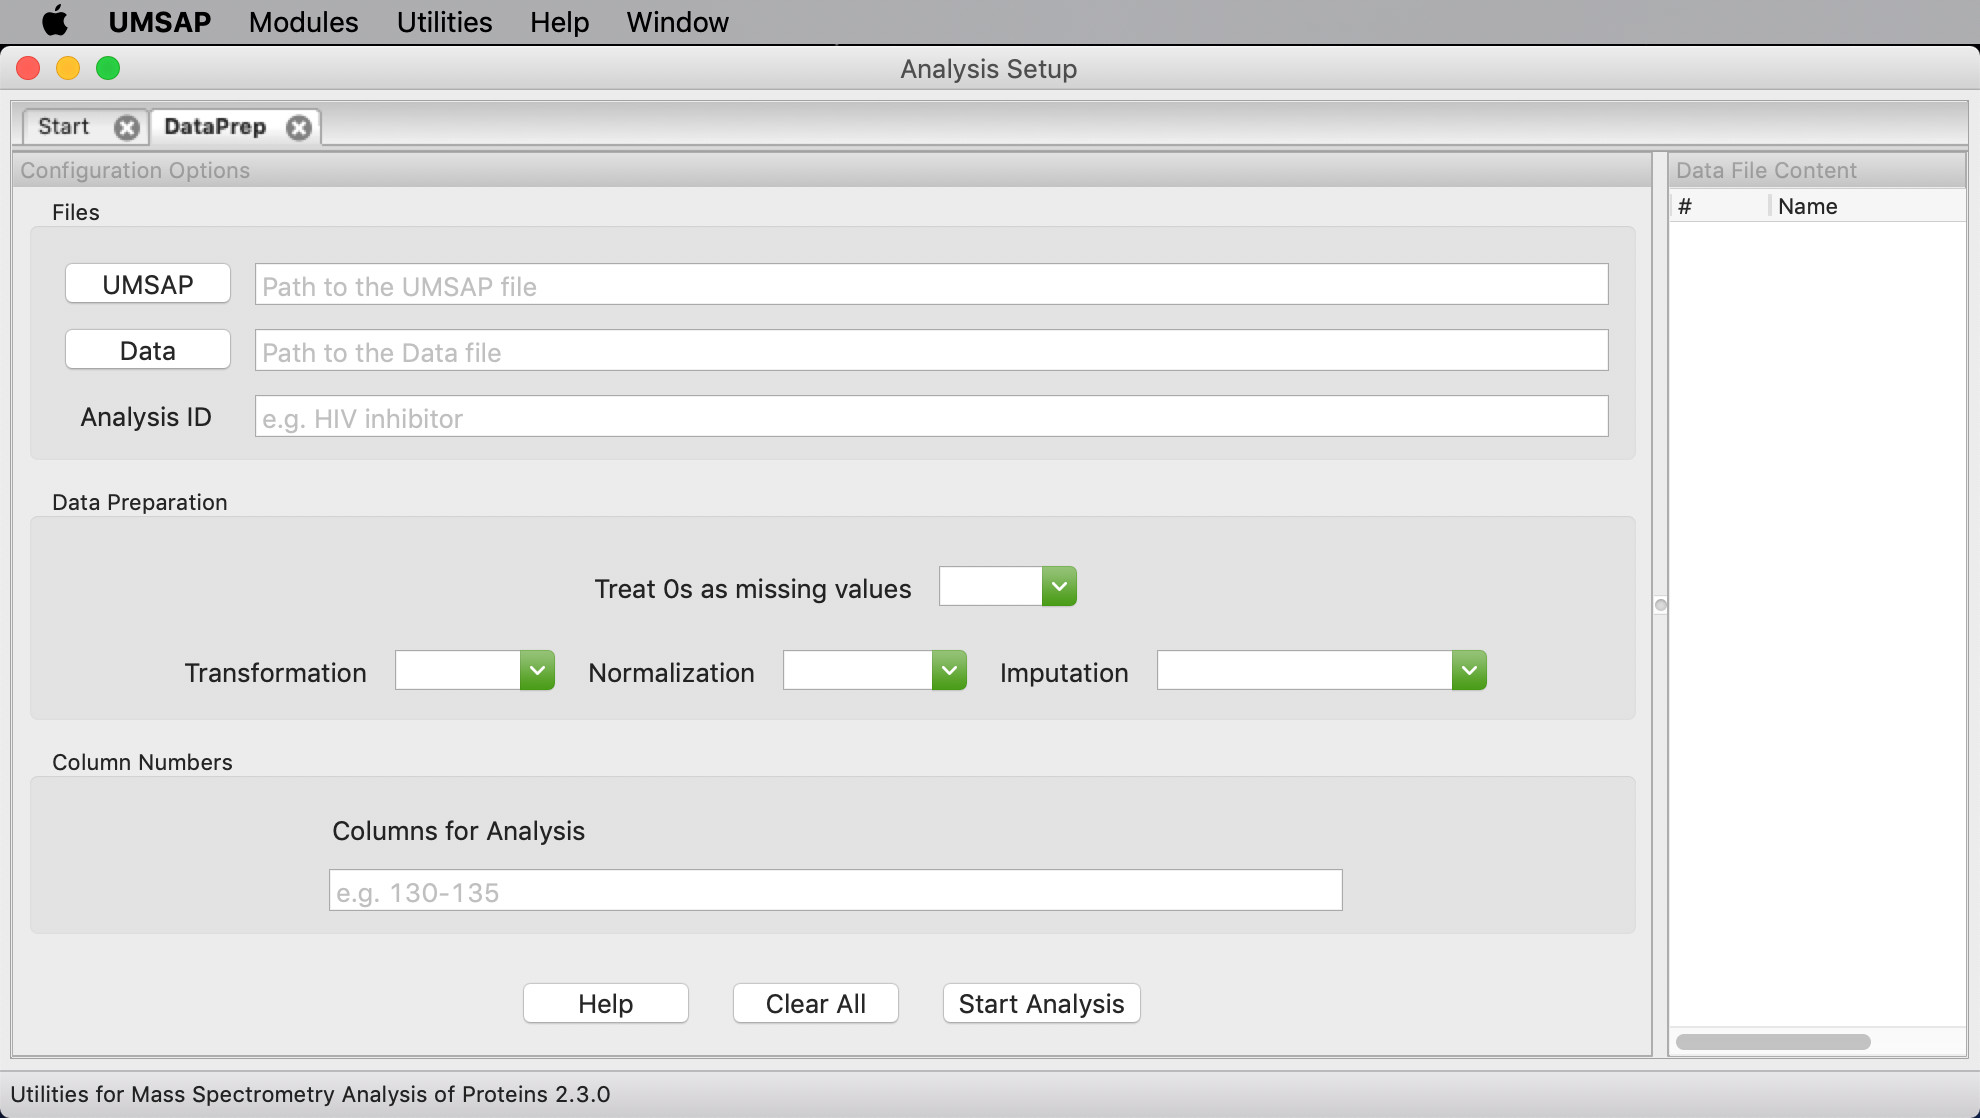
\includegraphics[width=0.7\textwidth]{./IMAGES/DATAPREP/DataPrep.jpg}
    \caption[The Data Preparation tab]{\textbf{The Data Preparation tab.}
    This tab allows performing a statistical exploration of the data contained in
    a given Data file.} 
    \label{fig:dataPrepTab}
    \vspace{-5pt}
\end{figure}

Region Data File Content holds a table to show the name of the columns in
the selected Data file. The table will be automatically filled after selecting the
file. Selected rows in the table can be copied (Cmd+C) and pasted (Cmd+V) to the
text fields in region Configuration Options.

Region Configuration Options contains all the fields needed to configure and
run the analysis. 

Section Files contains two buttons and a text field. Here users select the input
and output files for the analysis.

\num{1}. The button UMSAP allows selecting the location
and name of the umsap file. When selecting an already existing umsap file the operating
system will ask if it is ok to replace the file, the answer can be yes since UMSAP
will never overwrite or replace an umsap file. Instead, the new analysis will be
added to the already existing file. Only umsap files can be selected here.

\num{2}. The button Data allows selecting the input
data file that will be used for the analysis. The Data file is expected to be a
plain text file with tab separated columns and the name of the columns in the first
row of the file. In addition, columns to be analyzed must contain only numbers and
must be of the same length. Only .txt files can be selected here.

\num{3}. The text field Analysis ID allows providing an ID for the analysis
to be run. The date and time of the analysis will be automatically added to the
beginning of the name. For example, the Analysis ID \textit{First experiment} will
be transformed into \textit{20220504-124534 - First experiment}.

Section Data Preparation contains four dropdown boxes. Here users select the workflow
to be applied to the Data.

\num{1}. The dropdown Treat \num{0}s as missing values allows defining how
to handle zero values present in the Data file. Selecting Yes results in UMSAP
replacing zero values with NA values. Selecting No results in UMSAP considering
zeros as valid values.

\num{2}. The dropdown Transformation allows selecting the Transformation method
to be applied to the data.

\num{3}. The dropdown Normalization allows selecting the Normalization method
to be applied to the data.

\num{4}. The dropdown Imputation allows selecting the Imputation method used
to replace missing values in the data. The Imputation method Normal Distribution
requires specifying two additional parameters. The parameters Shift control the
center of the normal distribution used to randomly generate the missing values
while the parameter Width control the standard deviation of the distribution.

Section Column numbers contains a text field. Here users specify the Columns in the
Data file to be used during the Data Preparation steps. Only integers can be accepted
here. Column numbers can be copied (Cmd+C) and paste (Cmd+V) from the selected rows
in the table on region Data File Content or the numbers can be just typed.

The bottom of the region contains three buttons.

\num{1}. The button Help leads to an online tutorial about Data Preparation in
UMSAP.

\num{2}. The button Clear All will delete all user input from the tab.

\num{3}. The button Start Analysis starts the Data Preparation workflow.

\section{The analysis}

First, UMSAP will check the validity of the user-provided input. After this, the
selected Data file is read and the following steps are taken:

\num{1}. The content of all specified columns in Data file is checked to make sure
only numbers are found in them. \num{0} values present in the columns are left or
remove depending on the selected value for dropdown Treat \num{0}s as missing values.

\num{2}. The indicated Transformation method is applied to the selected columns.

\num{3}. The indicated Normalization method is applied to the transformed data.

\num{4}. The indicated Imputation method is applied to the normalized data.

The results from the four steps is saved, so users can check the effect of the selected
workflow over the data. Currently, only one method is implemented for the Transformation,
Normalization and Imputation of the data, respectively. The only alternative is to skip
the corresponding step. The methods available will be expanded in the near future.
All steps are column wise applied.

\section{The results window}

The window showing the results from a Data Preparation workflow is divided in three
regions (\autoref{fig:dataPrepRes}).

\begin{figure}[h]
    \centering
    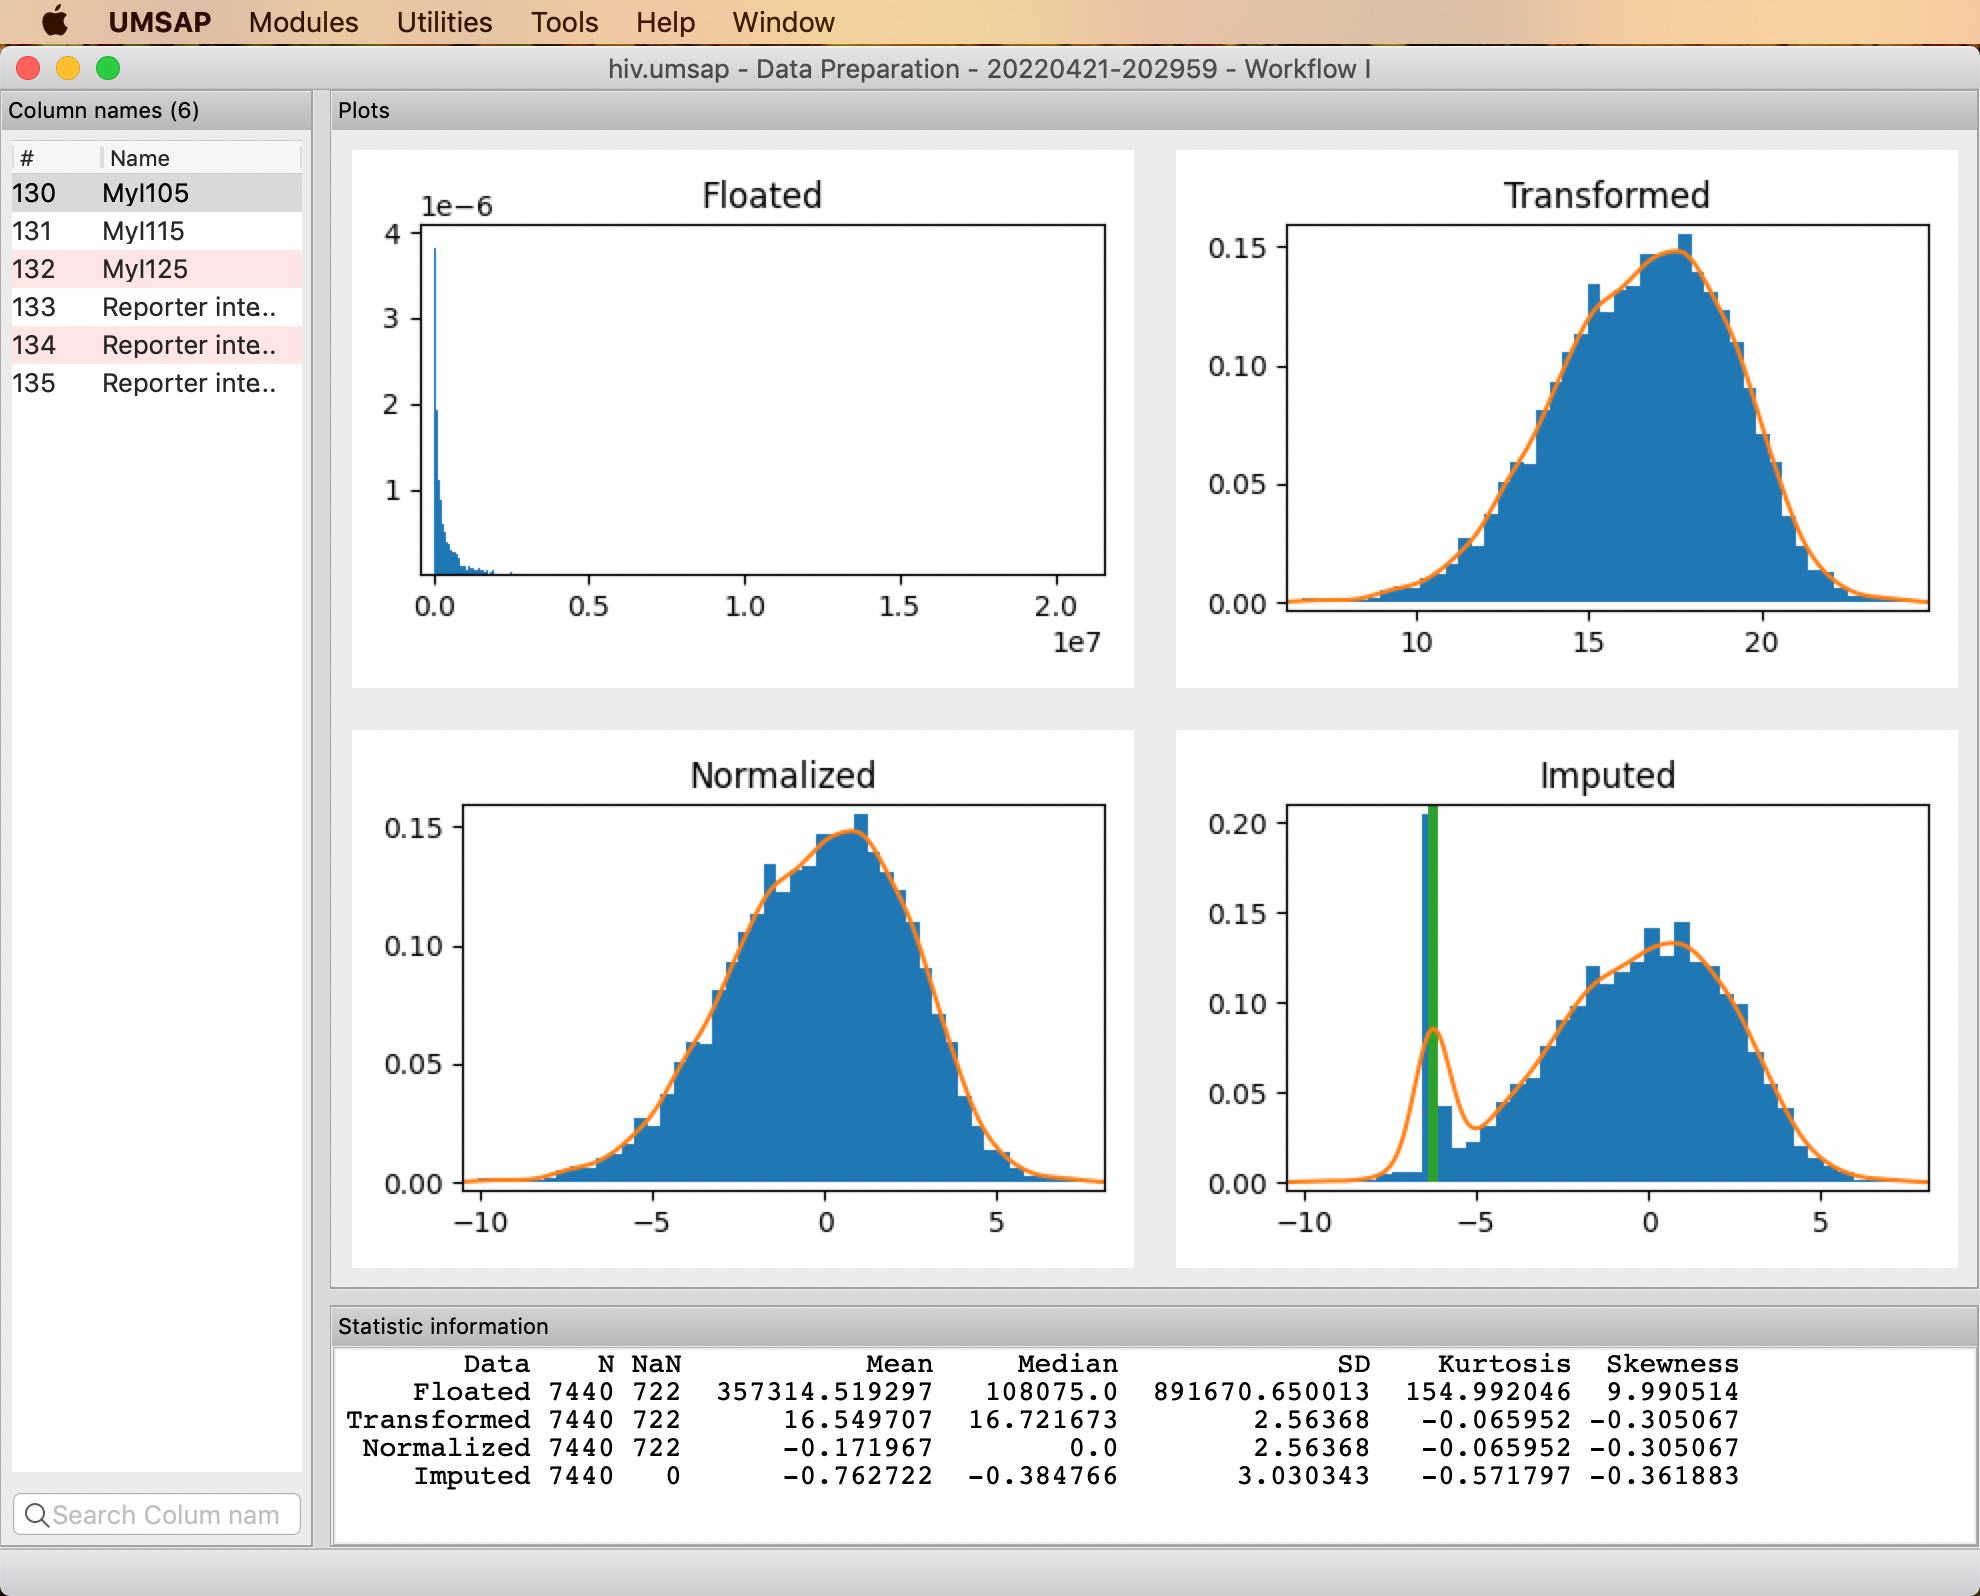
\includegraphics[width=0.7\textwidth]{./IMAGES/DATAPREP/DataPrepRes.jpg}
    \caption[The Data Preparation result window]{\textbf{The Data Preparation
    result window.} Histograms for the initial, transformed, normalized and
    imputed data are shown. }
    \label{fig:dataPrepRes}
    \vspace{-5pt} 	
\end{figure} 

Region Column names shows a table with the number (\num{0} based) and name of the
analyzed columns. 

Region Plots shows the results from the Data Preparation workflow in four histograms
for the selected column in region Column names. The histograms are created for the
initial, transformed, normalized and imputed data. They show the probability density
as blue bars and the calculated probability density function in orange. The green bars
in the Imputed histogram represent the imputed values.

Region Statistic information shows a description of the data for the selected column
in region Column names.

\section{The Tools menu}

The menu Tools in the window showing the results from a Data Preparation workflow
allows viewing any of the Data Preparation analyzes contained in the selected
umsap file. The menu Tools also allows duplicating the window (Cmd+D) for easier
comparison of two or more set of results, creating an image of the plots (Alt+Shift+I),
exporting the data shown to a tab separated CSV file (Cmd+E) and resetting the zoom
level of the plots (Alt+Shift+Z).